\chapter{Divers}
\label{chap:divers}

    Dans cette partie nous avons voulu présenter une partie du travail que nous avons fourni et qui ne rentrait pas dans la partie principale (les tests JUnit~\ref{chap:JUnit} et la comparaison entre le harnais et JUnit~\ref{chap:comparaison}), notamment les retours que nous avons fait par rapport à des bugs.

\section{Bugs}
    Au cours de notre travail avec COSTOTest nous avons été confrontés à plusieurs bug que nous avons remontés mais pour lesquels nous n'avons pas pu fournir de correctif.
        
    \subsection*{Génération incomplète}
    Lorsqu'on génère un harnais de test en utilisant \textit{Generate and Launch TH}, le package mylib nécessaire à une partie du code généré n'est lui-même pas généré.\footnote{Ce package n'est pas non plus généré lors de l'utilisation de Kml2java}
    
    Pour éviter ce bug, il suffit de lancer l'opération de génération sans la mener à sa fin puis de faire \textit{Laucnh TH} sur la classe TH\_PlatoonTestIntention.kcp qui va générer le package mylib. 

    \clearpage
    
    \subsection*{Menu Harness}
    Nous avons constaté un bug mineur lors de l'utilisation de la création de harnais, si jamais on ouvre le menu Harness et qu'on clique sur quit, ça ferme complètement Eclipse au lieu de juste quitter la création de harnais.

    \begin{figure}[H]
        \begin{center}
          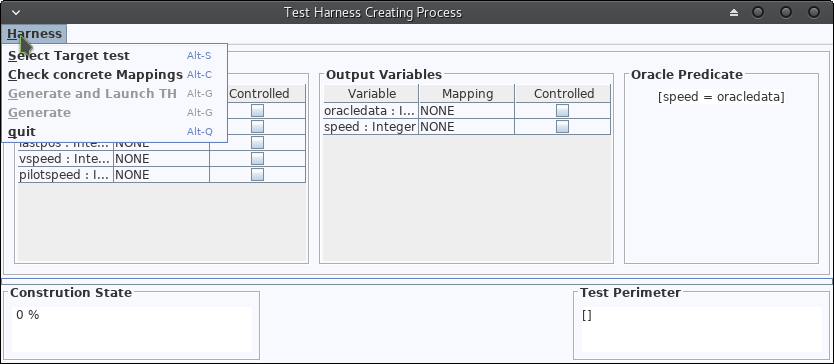
\includegraphics[scale=0.45]{images/bugquitter.png}
        \end{center}
    \end{figure} 
    
    \subsection*{Nom de véhicule bloquant}
    
    Lorsqu'on utilise \textit{Generate TH M2Alma}, si on sélectionne \textit{Select Target Test} dans le menu \textit{TestHarness Creating Process} et qu'on sélectionne SimpleVehicle avec comme seul paramètre computespeed et qu'on cherche à assigner une valeur au String vname puis qu'on annule sans valider le nom du Vehicle, il devient impossible d'assigner un String vname. La fenêtre ne réapparaît plus et le boutont devient inutilisable, nécessitant un redémarrage d'Eclipse pour pouvoir à nouveau travailler avec.

